\chapter{Simulation-based inference} \label{cha:sbi}
	
The purpose of this chapter is to complement the introduction by laying the foundations of the simulation-based statistical inference framework employed throughout the rest of the thesis. First, we provide an overview of traditional and neural network-based \gls*{sbi} implementations. Then, we focus on the specific algorithm that will be employed in the following chapters of this thesis, truncated marginal neural ratio estimation. We will then compare it with the other core \gls*{sbi} algorithms, highlighting advantages and pitfalls. Finally, we will outline this thesis specific contribution to the \gls*{sbi} field for astrophysical data analysis.


\section{The landscape of \gls*{sbi}} \label{sec:sbi}

In this section, we describe the developments and landscape of \gls*{sbi} algorithms. We begin in Section \ref{subsec:abc} by providing a brief overview of traditional implicit-likelihood methods for posterior inference, approximate bayesian computation \cite{Sisson:2018aa} and kernel density estimation \cite{diggle1984monte}. We then explain in Section \ref{subsec:nsbi} the different routes one can use to vastly accelerate and scale this process using neural networks \cite{Cranmer:2019eaq, Lueckmann:2021aa}. A comparison of the various neural \gls*{sbi} algorithms with a discussion about their drawbacks and advantages can be found later in Section \ref{sec:comparison}. 

%Turning more towards the history and development of \gls*{sbi}, there are two common traditional approaches that use simulations to do statistical inference when the analytic form of the likelihood is intractable. 


\subsection{Traditional \gls*{sbi}}  \label{subsec:abc}

The first implicit-likelihood ideas date back to the 1980s. Particularly relevant for the initial development of this paradigm was statistician Donald Rubin's discussion about the use of frequency calculations for the interpretation of Bayesian statements \cite{rubin1984bayesianly}. Importantly, in these lectures he encouraged statisticians to not settle for analytically tractable models only, but to instead consider computational methods to estimate the posterior distribution of interest for a wider range of models. An outline of the most well-known traditional \gls*{sbi} algorithm, \gls*{abc}, can be already found in Rubin's work \cite[Section 3.1]{rubin1984bayesianly}. 


\subsubsection{Approximate bayesian computation}

It is worth exploring in more details the \gls*{abc} algorithm, since it will serve us as the classical analogue of the \gls*{sbi} technique mostly employed throughout this thesis (see Section~\ref{sec:tmnre}). For more detailed reviews see Refs.~\cite{marin2012approximate, Sisson:2018aa, Grazian:2019aa}. \Gls*{abc} is a rejection sampling algorithm where, given a prior $\param\sim p(\param)$ proposed samples $\data \sim p(\data\mid\param)$ from the forward model are compared to the target observed data $\data_0$ with a hand-crafted distance measure based on some low-dimensional summary statistics $s(\data)$, as for example
\begin{equation}
    d(\data, \data_0)  = \| s(\data) - s(\data_0)\|\;.
\end{equation}
Samples from the approximate posterior are drawn with rejection sampling using an acceptance tolerance $\epsilon$ such that samples satisfy $d(\data, \data_0) < \epsilon$.
Hence the posterior
\begin{equation}
    p_\text{ABC}(\param\mid\data) = \frac
    {\int_{d(\data_0, \data) < \epsilon} d\data\, p(\param\mid\data)p(\data)}
    {\int_{d(\data_0, \data) < \epsilon} d\data\, p(\data)} \;
\end{equation}
is guaranteed to converge to the true one for sufficiently informative summary statistics $s(\data)$ and for $\epsilon \to 0$, $p_\text{ABC}(\param\mid\data) \xrightarrow{\epsilon \to 0} p(\param\mid\data)$. Whereas, when $\epsilon$ is non-zero, the approximate posterior is guaranteed to be broader than the true one, leading to conservative inference. 

Interestingly, a physical implementation of \gls*{abc}-rejection scheme for a single parameter and a single observation was already constructed by Francis Galton in the late 1800s \cite[Figure 5]{stigler2010darwin}. The device is known today as the Galton board, and often used to demonstrate the central limit theorem \cite{galton1889natural}. Since Rubin's work, \gls*{abc} has been widely adopted in astrophysics and cosmology, including applications to, \eg, galaxy demographics \cite{cameron2012approximate}, galaxy–halo connection \cite{hahn2017approximate}, intergalactic medium \cite{Davies:2017eir}, exoplanetary systems \cite{hsu2018improving}, luminosity functions \cite{Riechers:2018zjg}, stellar initial mass function \cite{cisewski2019preferential}, cosmology \cite{Akeret:2015uha, jennings2017astroabc}, galaxy clustering \cite{Ishida:2015wla}, type Ia supernovae \cite{Weyant:2012xe}, gamma-ray sky \cite{Baxter:2021tui}, and cosmic rays \cite{bourriche2024beyond}. The quick adoption of \gls*{abc} from the astrophysical community has also been accompanied by the development of specialized software, which have played an important role in the dissemination of the technique such as \texttt{CosmoABC} \cite{Ishida:2015wla}, \texttt{abcpmc} \cite{Akeret:2015uha}, and \texttt{astroABC} \cite{jennings2017astroabc}.


\subsubsection{Approximate frequentist computation}

A second classical approach to \gls*{sbi} was also proposed in the 1980s by Diggle and Gratton \cite{diggle1984monte}. The approach was dubbed ``approximate frequentist computation" by the authors of Ref.~\cite{brehmer2018guide} because of its similarities to \gls*{abc}. Specifically, this method is based on creating an approximate model for the likelihood by estimating the distribution of low-dimensional summary statistics from samples drawn from the simulator with histograms or \emph{kernel density estimation}. The advantage over \gls*{abc} is that it is amortized, meaning that after the initial computational cost for the simulation and density estimation phase, evaluating new data points becomes efficient \todo{Is this true? From Cranmer review. But thought ABC is amortized}.
This property makes kernel density estimation-based inference particularly well suited for problems with many i.i.d. observations, a key reason for its widespread use in particle physics measurements \cite{Brehmer:2020cvb}. For example, this approach was used for the discovery of the Higgs boson in a frequentist paradigm \cite{brehmer2018guide}. 


\subsubsection{Moving \gls*{sbi} forward}

Despite their success and continuous progresses, there are some explicit disadvantages of these classical \gls*{sbi} methods (of which the community is aware of \cite[see \eg][]{Trotta:2017wnx}), that makes them unsuitable for high-dimensional and complex data. First, they both rely on low-dimensional summary statistics $s(\data)$ to compare simulations to the data, which may not retain all the information available in the data. Second, they suffer from the curse of dimensionality, with a required simulation budget that increases with the dimensionality of the parameter space \cite[\eg][]{Leclercq:2018who}. In particular, the acceptance rate of \gls*{abc}'s rejection algorithm vanishes exponentially as the dimensionality of the parameter space increases, thus significantly more simulation budget is needed to reach convergence in high dimensions for $\epsilon \to 0$.

These challenges are tackled in modern \gls*{sbi} algorithms thanks to advances in deep learning \cite{lecun2015deep} and automatic differentiation \cite{baydin2018automatic}. In particular, first, the development of neural network's architectures tailored to various data structures has been fundamental for the processing of significantly more complex data  \cite{lecun2015deep}. This allows for the optimization of learned data features w.r.t. some custom loss, instead of relying on hand-crafted summary statistics. Second, neural network-based algorithms are being actively developed to estimate probability density distributions in high dimensions, overcoming the curse of dimensionality \cite[\eg][]{papamakarios2019neural, papamakarios2021normalizing, Papamakarios:2016ctj}. In the next section, we will discuss the main neural network-based \gls*{sbi} algorithms. 


\subsection{Neural \gls*{sbi}} \label{subsec:nsbi}

Moving beyond the classical \gls*{sbi} approaches, in recent years, a number of new neural network-based \gls*{sbi} techniques have been proposed. We refer the reader to Ref.~\cite{Cranmer:2019eaq} for a general review, to Ref.~\cite{Lueckmann:2021aa} for benchmarks of the various algorithms, and to Ref.~\cite{Ho:2024whi} for an exhaustive comparisons of all \gls*{sbi} methods currently available as well as discussions about their challenges and pitfalls in the context of astrophysics and cosmology.\footnote{An extensive list of works that use neural \gls*{sbi} in astrophysics, cosmology, and high energy physics can be found here: \url{https://github.com/smsharma/awesome-neural-sbi}.}
The widespread adoption of these methods in astrophysics and cosmology has also been driven by the development of specialized tools, such as, \eg, \texttt{pydelfi} \cite{Alsing:2019xrx}, \texttt{sbi} \cite{tejero-cantero2020sbi}, \texttt{swyft} \cite{Miller2022}, and \texttt{lampe} \cite{lampe}. 

In general, Bayes' theorem (Equation~\eqref{eq:sbi-Bayes}) hints at a few different approaches for the implementation of neural \gls*{sbi} algorithms: \gls*{npe} which employs density estimation techniques to directly estimate the posterior $p(\param\mid\data)$ \cite{Papamakarios:2016ctj, Greenberg:2019aa}; \gls*{nle} which instead uses density estimation to learn an approximation to the likelihood $p(\data\mid\param)$ \cite{Papamakarios:2018aa, Durkan:2018aa}; and \gls*{nre} \cite{cranmer2015approximating, gutmann2018likelihood, Hermans:2019ioj, thomas2022likelihood, Miller:2020hua} which uses classifiers to approximate the likelihood-to-evidence or posterior-to-prior ratio $\frac{p(\data\mid\param)}{p(\data)}=\frac{p(\param\mid\data)}{p(\param)}$. In the following paragraphs, we will describe their fundamental properties.


\subsubsection{Neural posterior estimation}

\Gls*{npe} is the most straightforward method \cite{Papamakarios:2016ctj, Greenberg:2019aa}. It introduces a density estimator $q^\text{VI}_\Phi(\param\mid\data)$, parametrized through the weights $\Phi$, which is trained to approximate the posterior for parameters $\param$ given data $\data$,
%
\begin{equation}
    q^\text{NPE}_\Phi(\param \mid \data) \approx p(\param\mid\data)\;.
\end{equation}
%
Specifically, we want to reduce the dissimilarity between the density estimator $q^\text{NPE}_\Phi(\param \mid \data)$ and the true posterior $p(\param\mid\data)$ by minimizing w.r.t.~the weights $\Phi$ the \emph{forward} \gls*{kl} divergence \cite{Kullback:1951zyt},
%
\begin{align} \label{eq:fkl}
%\mathop{\arg\min}\limits_\Phi
	D_{\mathrm{KL}}(p \| q^\text{NPE}_\Phi) &= \int \dd \param \,p\left(\param \mid \data\right) \ln \left(\frac{p\left(\param \mid \data\right)}{q^\text{NPE}_\Phi\left(\param \mid \data\right)}\right) \\
	& =\mathop{\mathbb{E}}\limits_{\param \sim p\left(\param \mid \data\right)}\left[\ln \frac{p\left(\param \mid \data\right)}{q^\text{NPE}_\Phi\left(\param \mid \data\right)}\right]
\end{align}
%
%\begin{equation} \label{eq:kld}
%    D_{KL}(p(x) \mid q(x) = \sum_{x} p(x) \log\left(\frac{p(x)}{q(x)}\right) \;.
%\end{equation}
%
As the expectation value is taken over samples from the true posterior distribution, we cannot evaluate the above quantity. To overcome this limitation, one averages over simulation data $\data \sim p(\data)$. The loss is now the expected forward \gls*{kl} divergence, where we have exploited the fact that $p(\param\mid \data) p(\data)=p(\data, \param)$, which we know how to sample:
%
\begin{align}
	\mathop{\mathbb{E}}\limits_{\data \sim p(\data)}\left[D_{\mathrm{KL}}(p \| q^\text{NPE}_\Phi)\right] & =\mathop{\mathbb{E}}\limits_{\data, \param \sim p(\data, \param)}\left[\ln \frac{p(\param \mid \data)}{q^\text{NPE}_\Phi(\param \mid \data)}\right] \\
	& =\underbrace{-\mathop{\mathbb{E}}\limits_{\data, \param \sim p(\data, \param)} \ln q^\text{NPE}_\Phi(\param \mid \data)}_{\text{expected entropy}}+\underbrace{\mathop{\mathbb{E}}\limits_{\data, \param \sim p(\data, \param)} \ln p(\param \mid \data)}_{\text {constant}} \;.
\end{align}

\Gls*{npe} loss function is then given by the negative log-probability
%
\begin{equation} \label{eq:lnpe}
	\mathcal{L}^\text{NPE}=-\mathop{\mathbb{E}}\limits_{\data, \param \sim p(\data, \param)} \ln q^\text{NPE}_\Phi(\param \mid \data) \;.
\end{equation}
%
Application of this loss function requires that the density estimator is normalized to one, $\int \dd\param\ q^\text{NPE}_\Phi(\param \mid \data)=1$, which can be guaranteed by using specific network architectures to parametrize $q^\text{NPE}_\Phi$. The most popular ones with this property are normalizing flows, which transform tractable density functions into complex ones through a sequence of invertible operations with tractable Jacobians \cite{kobyzev2020normalizing, papamakarios2021normalizing}. The \gls*{npe} algorithm has the advantage that it allows both for evaluation and sampling of the estimates the posterior from the normalizing flow. However, the pitfall is that it requires an analytic form of the proposal prior from which training data was sampled, which may not be always accessible (\eg\ from cosmological simulations).

\Gls*{npe} has been widely used in astrophysics, \eg, for strong gravitational lensing analysis \cite{Wagner-Carena:2020yun, Wagner-Carena:2022mrn, wagnercarena2024strong}, gravitational waves parameter estimation \cite{Dax:2021tsq, Crisostomi:2023tle, kolmus2024tuning}, gravitational wave background reconstruction \cite{Dimitriou:2023knw}, cosmological parameter inference \cite{Tucci:2023bag}, X-ray spectral fitting \cite{Barret:2024kvc}, exoplanetary atmospheric retrieval \cite{vasist2023neural}, galaxy spectra inference \cite{Hahn:2022nda, khullar2022digs}, galactic center $\gamma$-ray excess characterization \cite{Mishra-Sharma:2021oxe, Christy:2024hou}, among other applications.

\paragraph{Comparison with variational inference} 
It is interesting to compare \gls*{npe} with its direct likelihood-based counterpart, variational inference \gls*{vi} (for a review see Ref.~\cite{zhang2018advances}), already mentioned in \todo{add}. \Gls*{vi} allows the approximation of extremely high-dimensional Bayesian posteriors with simple proposal distributions by solving an optimization problem. 
This is achieved by using a proposal distribution, the so-called variational posterior, $q^\text{VI}_\Phi(\param \mid \data_0)$, to approximate the true posterior $p\left(\param \mid \data_0\right)$ and optimizing its parameters $\Phi$ using gradient ascent \cite{Murphy:book, bottou:nips, kingma2014adam}. \Gls*{vi}'s optimization objective is the \emph{reverse} \gls*{kl} divergence
%
\begin{align} \label{eq:rkl}
	D_{\mathrm{KL}}(q^\text{VI}_\Phi \| p)  &= \int \dd \param\; q^\text{VI}_\Phi\left(\param \mid \data_0 \right) \ln \left(\frac{q^\text{VI}_\Phi\left(\param \mid \data_0\right)}{p\left(\param \mid \data_0\right)}\right) \\
	& =\mathop{\mathbb{E}}\limits_{\param \sim q^\text{VI}_\Phi\left(\param \mid \data_0\right)}\left[\ln \frac{q^\text{VI}_\Phi\left(\param \mid \data_0\right)}{p\left(\param \mid \data_o\right)}\right]
\end{align}
%
Similarly to the trick used for \gls*{npe}, in order to avoid evaluating the inaccessible posterior $p\left(\param \mid \data_o\right)$, one exploits Bayes' theorem and substitute $p(\param| \data) = p(\data| \param) p(\param) / p(\data)$, obtaining:
%
\begin{align}
	D_{\mathrm{KL}}(q^\text{VI}_\Phi \| p) &=
	\mathop{\mathbb{E}}\limits_{\param \sim q^\text{VI}_\Phi(\param \mid \data_o)}\left[\ln \frac{q^\text{VI}_\Phi(\param \mid \data_o)}{p(\param \mid \data_o)}\right] \\
	& =\underbrace{\mathop{\mathbb{E}}\limits_{\param \sim q^\text{VI}_\Phi(\param\mid \data_o)}\left[\ln \frac{q^\text{VI}_\Phi(\param \mid \data_o)}{p(\data_0 \mid \param) p(\param)}\right]}_{\equiv-{\rm ELBO}}+ \underbrace{\ln p(\data_0)}_\text{constant} \;,
\end{align}
%
where we have introduced the evidence lower bound (ELBO). Minimizing the reverse \gls*{kl} divergence is thus equivalent to maximizing the ELBO, and the \gls*{vi} loss is
%
\begin{equation} \label{eq:lvi}
	\mathcal{L}^\text{VI} = -\mathrm{ELBO} \equiv {\mathop{\mathbb{E}}\limits_{\param \sim q^\text{VI}_\Phi\left(\param \mid \data_0\right)}\left[\ln p\left(\data_0, \param\right)-\ln q^\text{VI}_\Phi\left(\data_0 \mid \param\right)\right]} \;.
\end{equation}

We can now comment upon the main differences between \gls*{npe} and \gls*{vi}. First, in \gls*{npe} parameters are drawn from the model prior $p(\param)$ (see Equation~\eqref{eq:lnpe}), whereas in \gls*{vi} they are drawn from the variational posterior $q^\text{VI}_\Phi\left(\param \mid \data_0\right)$ (see Equation~\eqref{eq:lvi}). As a result, in the latter case, samples increasingly focus on regions with high data likelihood $p(\data_o \mid \param)$, whereas in \gls*{npe} there is no  automatic focusing on regions with high data likelihood. Second, for \gls*{vi} the posterior  $q^\text{VI}_\Phi\left(\param \mid \data_0\right)$ must cover all parameters that the likelihood model is conditioned on, and omitting correlations (\eg\ mean-field approximation) gives a lower bound on parameter uncertainties. On the other hand, in \gls*{npe}, if we substitute $q^\text{NPE}_\Phi(\param\mid\data)$ with a low dimensional marginal, \eg\ $q^\text{NPE}_\Phi(\Theta_1\mid\data)$, we automatically get marginal posterior estimates, without performing integrals explicitly. Hence, omitting correlations generates correctly marginalized posteriors \cite{ambrogioni2019forward}. The ability to directly perform marginal inference is shared among all other neural \gls*{sbi} algorithms, and it is one of the main differences with likelihood-based algorithms. 


\subsubsection{Neural likelihood estimation}

Another choice for neural \gls*{sbi} is to perform {\gls*{nle}} \cite{Papamakarios:2018aa, Durkan:2018aa}, where one trains an estimator for the likelihood probability density of the data $\data$ given some model parameters $\param$, 
\begin{equation}
    q^\text{NLE}_\Phi(\data \mid \param) \approx p(\data\mid\param)\;.
\end{equation}
Following a similar reasoning as the one employed to derive \gls*{npe} loss function, \gls*{nle} loss function is given by the negative log-likelihood
%
\begin{equation}
	\mathcal{L}^\text{NLE}=-\mathop{\mathbb{E}}\limits_{\data, \param \sim p(\data, \param)} \ln q^\text{NLE}_\Phi(\data \mid \param) \;.
\end{equation}
%
Again, specialized network architectures as normalizing flows are typically employed to guarantee that $q^\text{NLE}_\Phi(\data \mid \param)$ is a properly normalized density function.

As a general guideline, the choice between \gls*{npe} or \gls*{nle} for different physical problems should consider the dimensionality of the data and parameter space, as well as the complexity of learning likelihood or posterior distribution's shape. Indeed, neural networks are easier to train when using high-dimensional input to yield low-dimensional output than vice versa. Thus, if the data is high-dimensional (\eg, images), then \gls*{npe} may be a more suitable choice than \gls*{nle}. Conversely, for high-dimensional posterior inference (\ie, when the dimension of the parameter space is large), \gls*{nle} often outperforms \gls*{npe}, especially when there are strong parameter degeneracies. 

\Gls*{nle} has also been widely used in astrophysics, for gravitational waves parameter estimation \cite{Vilchez:2024qnw} and cosmological parameter inference \cite{Alsing:2019xrx, Modi:2023drt, Makinen:2021nly, DES:2024xij, Jeffrey:2020aa, vonWietersheim-Kramsta:2024cks}, among other applications.


\subsubsection{Neural ratio estimation}

Bayes' theorem hints at a last quantity that can be estimated, the likelihood-to-evidence or posterior-to-prior ratio 
\begin{equation}
	r(\param;\data)\approx\frac{p(\data\mid\param)}{p(\data)}=\frac{p(\param\mid\data)}{p(\param)}\; .
\end{equation}
This quantity is approximated using binary classification via a supervised learning task. In this case, the ratio does not need to be normalized, hence one is free to use any neural network architecture. 

We will explore in more details the \gls*{nre} algorithm in a dedicated section, Section~\ref{subsec:tmnre-nre}, as in this thesis we will focus on this last method and its extensions. Moreover, a detailed comparison between \gls*{nre} and its extension with the other neural \gls*{sbi} algorithms is presented in Section~\ref{sec:comparison}.

\Gls*{nre} has also been widely used in astrophysics and cosmology, for gravitational waves parameter estimation \cite{Bhardwaj:2023xph, Alvey:2023naa}, gravitational wave background reconstruction \cite{Alvey:2023npw}, strong gravitational lensing analysis \cite{Montel:2022fhv,  Coogan:2022cky, Brehmer:2019jyt, Zhang:2022djp}, cosmology \cite{List:2023aa, Cole:2021gwr, FrancoAbellan:2024tbj}, stellar streams analysis \cite{Hermans:2020skz, albatross}, 21-cm power spectra \cite{Saxena:2023tue}, type Ia supernovae \cite{Karchev:2022xyn, Karchev:2024stw}, point source detection \cite{AnauMontel:2022ppb}, millisecond pulsars \cite{Berteaud:2024zda}, astrometry \cite{Mishra-Sharma:2021nhh}, among other applications. 


\subsubsection{Active learning} There are a number of additional features that can be used on top of these core \gls*{sbi} algorithms, either preceding or following the main inference step. Here, we further refine the taxonomy of \gls*{sbi} algorithms based on whether they use some form of {active learning} to guide the simulator towards parts of the parameter space that are most relevant for a specific target observation $\data_0$. In particular, \emph{sequential} \gls*{sbi} approaches adaptively choose informative simulations by using sequentially refined proposal distributions for the model parameters. They have been reported to outperform and be more simulation-efficient with respect to non-sequential ones across a number of different benchmark tasks \citep{Lueckmann:2021aa} and, \eg, in cosmology \cite{Cole:2021gwr}, in gravitational waves astrophysics \cite{Bhardwaj:2023xph}, and in strong lensing analysis \cite{wagnercarena2024strong}. Particularly impressive is the recent result form Ref.~\cite{wagnercarena2024strong}, where they perform a sequential \gls*{npe} analysis of strong gravitational lenses, that would have taken 2000 times longer without the use of active learning \cite[Figure 5 in][]{wagnercarena2024strong}.

The core intuition behind sequential \gls*{sbi} algorithms is the following: given a single observation of interest, $\data_0$, sampling parameters from the entire prior space to generate training data may not be efficient, since it leads to training data $(\data, \param)$ that has significant variance compared to the target observation $\data_0$. Therefore, for a fixed simulation budget, the training samples contain only limited information about the posterior $p(\param\mid\data_0)$. The alternative proposed by sequential algorithms, in order to increase simulation efficiency, is to draw parameters from an adaptive proposal distribution $p^{(R)}(\param)$, resulting in training data that matches the observation of interest more closely in each sequential round $R$. More details regarding various possible implementations of sequential inference are given in Section~\ref{subsec:tmnre-t}.

\medskip

In this section we have introduced the core neural \gls*{sbi} algorithms. After describing in details the algorithm mostly employed in this thesis (Section~\ref{sec:tmnre}), we will compare it to the other ones in Section~\ref{sec:comparison}.


\section{Truncated Marginal Neural Ratio Estimation} \label{sec:tmnre}

We will now focus our attention on the main \gls*{sbi} technique employed in this thesis, \gls*{tmnre}. We provide a pedagogical introduction, and show that it forms the core of a fast, accurate and precise approach to solve general parameter inference problems in high-dimensional settings \cite{Miller:2020hua, Miller:2021aa, Miller:2022shs}. The approach builds on three key simple ingredients. First, neural ratio estimation (NRE). Second, focus on marginal inference (M).  Third, active learning through prior truncation (T).  We provide a technical description of them in the following sections, emphasizing how they compose well together.

\subsection{Neural Ratio Estimation: ``classification is all you need"} \label{subsec:tmnre-nre}

Ratio estimation rephrases Bayesian posterior inference as a binary classification problem.
Given an implicitly defined model $\data, \param \sim p(\data, \param) = p(\data\mid\param)p(\param)$, the idea behind ratio estimation is to use a binary classifier to distinguish between data \data\ and parameter \param\ pairs  drawn from two classes labeled by the binary variable $C$:
\begin{align}
    p(\data, \param  \mid C = 1) &= p(\data, \param ) \\
    p(\data, \param  \mid C = 0) &= p(\data) p(\param ) \, .
\end{align}
Concretely, these two distributions correspond respectively to drawing data and parameters jointly from the simulator, $\data, \param \sim p(\data, \param)$, or to drawing data and parameters marginally, $\data, \param \sim p(\data) p(\param)$, by sampling an unrelated set of parameters from the prior versus data from the simulator (this can be simply obtained by scrambling the joint pairs).\footnote{Throughout this thesis we will refer to joint samples as \emph{positive} training examples, and to marginal samples as \emph{negative} training examples.} 

Sampling $C=0$ and $C=1$ with equal probability, the decision function for the Bayes-optimal classifier  \cite{Devroye:1996aa} (\ie~the one that minimizes the Bayesian risk of missclassification) is:
\begin{equation} \label{eq:sbi-classifier}
    p(C = 1 \mid \data, \param) = \frac{p(\data, \param)}{p(\data, \param) + p(\data) p(\param)} \equiv \sigma[ \log r(\param; \data)] \, ,
\end{equation}
where we introduced the sigmoid function $\sigma(y) \equiv 1 / (1 + e^{-y})$. Importantly, the equivalence in Equation~\eqref{eq:sbi-classifier}, often called the ``likelihood ratio trick" \cite[\eg][]{cranmer2015approximating, Brehmer:2019jyt}, shows how the Bayes-optimal classifier is related to the  posterior-to-prior, likelihood-to-evidence, or joint-to-marginal distribution ratio:
\begin{equation} \label{eq:sbi-ratio}
    r(\param;\data) \equiv \frac{p(\param \mid \data)}{p(\param)} = \frac{p(\data \mid \param)}{p(\data)} =  \frac{p(\data, \param)}{p(\data) p(\param)} \, .
\end{equation}

Thus, one can gain access to the posterior-to-prior ratio by training a classifier of joint versus marginal pairs, which are easily obtainable with a forward simulator, and subsequently use it for inference. In practice, as the first equality in Equation~\eqref{eq:sbi-ratio} suggests, if the prior is tractable, $r(\param;\data)$ gives direct access to the posterior density:  $p(\param \mid \data)=r(\param;\data)p(\param)$.  Alternatively, one can use $r(\param;\data)$ to weight prior samples, enabling posterior sampling even when the prior cannot be expressed in closed-form.

Often, both the data and the parameters are typically high-dimensional objects (\eg strong lensing images and the parameters of a population of dark matter substructures, or galaxy clustering measures and  cosmological initial conditions parameters), and therefore neural network-based classifiers that are able to process this complex data and be efficiently optimized are a necessary choice.
As proposed by Ref.~\cite{Hermans:2019ioj}, in \gls*{nre} the classifier in Equation~\eqref{eq:sbi-classifier} is a \gls*{nn},  $d_{\bm{\Phi}}(\data, \param)$, that takes as input a parameters-data pair and produces an estimate of the ratio $\hat{r}(\param;\data)$.\footnote{Throughout this chapter we will use the notation $\hat{\square}$ to indicate quantities estimated via \gls*{nn}.} 
The network parameters ${\bm{\Phi}}$ are optimized via stochastic gradient descent  \cite{Murphy:book, bottou:nips, kingma2014adam} to minimize the \gls*{bce} \cite{mao2023cross}:
\begin{equation}\label{eq:sbi-bce}
\begin{split}
    \mathcal{L}[d_{\bm{\Phi}}(\data, \param)] = &-\int \dd \data  \dd\param \left\{ p(\data, \param) \log d_{\bm{\Phi}}(\data, \param) ] \right. \\
    & \left. + p(\data) p(\param) \log\left[ 1 - d_{\bm{\Phi}}(\data, \param) \right] \right\}\; .
\end{split}
\end{equation}
Therefore, by training a neural network $d_{\bm{\Phi}}(\data, \param)$ to estimate $\hat{r}(\param; \data)$ via this supervised classification task, we obtain an estimate of the posterior through $\hat{p}(\param \mid \data) = \hat{r}(\param; \data) p(\param)$. 

%Critically, training only requires the ability to generate \emph{samples} from the simulator. This makes it straightforward to apply ratio estimation in scenarios where the explicit form of the likelihood cannot be written in closed-form. 


\subsection{Marginalization: focus on the essentials} \label{subsec:tmnre-m} % zero-in on what matters, 

Joined posteriors are commonly a key component of a scientific workflow when analyzing real-world data, since access to joint posterior samples exhaustively solves a given Bayesian parameter inference. However, when the number of parameters becomes large (\eg, hundreds for a cosmic shear joint analysis of three surveys \cite{Piras:2024dml}, thousands for strong gravitational lensing substructures \cite{Montel:2022fhv, Coogan:2022cky} or background source reconstruction \cite{Karchev:2021fro}, or even millions for cosmological initial conditions \cite{Jasche:2012kq, List:2023aa}), the computational overhead of generating joint samples can be enormous. Furthermore, the full joint posterior $p(\param \mid \data)$ is usually only an intermediate step, and not the goal by itself: in many cases, scientific insight is based on a low-dimensional marginalization of the overly informative joint posterior over nuisance parameters.

Let us consider a model with a full joint distribution
\begin{equation}
	p(\data,\interest, \nuisance) = p(\data\mid\interest, \nuisance)p(\interest, \nuisance) \;,
\end{equation} 
where we have split the set of all model parameters $\param = \{\interest,\nuisance\} \in \mathbb{R}^D$ into parameters of interest $\interest \in \mathbb{R}^d$ (which we want to infer) and nuisance parameters $\nuisance \in \mathbb{R}^{D-d}$ (which we want to marginalize over). 
Formally, the marginal posterior is obtained by integrating the joint posterior over all nuisance parameters
\begin{equation}
	p(\interest \mid \data) = \int \dd\nuisance\ p(\interest, \nuisance \mid \data) \;.
\end{equation}


\begin{figure}
    \centering
	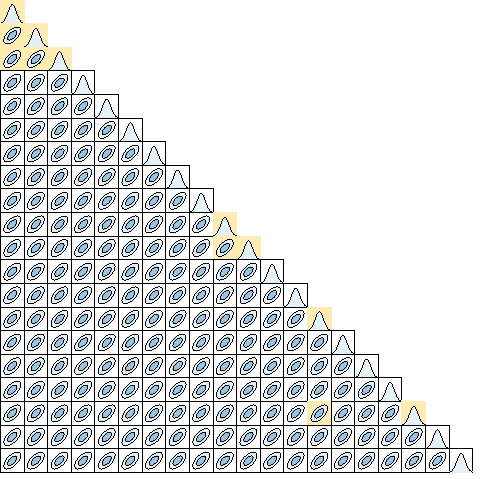
\includegraphics[width=\linewidth]{TikZ/corner.pdf}
    \caption{In simulation-based setting it is possible to directly estimate the marginal posterior of interest, instead of solving the problem for the full joint posterior at once, which can be computationally infeasible for complex models. Here we highlight some of the possible types of marginals that can be directly inferred in \gls*{sbi} for this mock high-dimensional parameter space.}
    \label{fig:sbi-marginals}
\end{figure}


Given the general \gls*{nre} setup, the extension to estimating marginal posteriors is straightforward: parameters to be marginalized over must be \emph{sampled}, but \emph{not presented} to the ratio estimator  \cite{Miller:2020hua}. Hence, marginalization over nuisance variables is done implicitly, since the data will incorporate the variance from the nuisance parameters, but the inference procedure estimates only the marginal likelihood-to-evidence ratio.

In more detail, if $\nuisance$ is not passed to the ratio estimator, the loss function becomes
\begin{align} 
   \mathcal{L}[d_{\bm{\Phi}}(\data, \interest)]&= -\int \dd\data \dd\interest \dd\nuisance\left\{ p(\data,\interest, \nuisance) \log d_{\bm{\Phi}}(\data, \interest,\nuisance) \right. \notag \\
    &\hspace{1.8cm} \left. + p(\data) p(\interest, \nuisance) \log\left[ 1 - d_{\bm{\Phi}}(\data, \interest,\nuisance) \right] \right\} \\
    &= -\int \dd{\data} \dd{\interest} \left\{ p(\data, \interest) \log d_{\bm{\Phi}}(\data, \interest) \right. \notag \\
    &\hspace{1.8cm} \left. + p(\data) p(\interest) \log\left[ 1 - d_{\bm{\Phi}}(\data, \interest) \right] \right\} \;, \label{eq:sbi-bce-m}
\end{align}
where we have integrated over $\nuisance$ to obtain the second equality, proving our statement. 
As a result, the binary classifier trained on $(\data, \interest)$ pairs effectively learns an estimate of the marginal likelihood-to-evidence ratios 
\begin{equation}\label{eq:sbi-ratio_marginal}
    \hat{r}(\data;\interest) \equiv \frac{p(\interest \mid \data)}{p(\interest)} =  \int \mathrm{d}\nuisance \, \frac{p(\boldsymbol{\theta, \eta} \mid \data)}{p(\interest)} p(\nuisance)  \, .
\end{equation}
We can then use the marginal ratio $\hat{r}(\data,\interest)$ to evaluate the marginal posterior for the parameters of interest directly or obtain samples otherwise, with significantly less computational cost. The possibility to directly access marginal posteriors can be easily obtained for  NLE and NPE density estimators as well \cite{Alsing:2019xrx, Jeffrey:2020itg}.

As touched upon in Section~\ref{sec:lbi-sbi}, this way of approaching the problem determines the scalability of \gls*{sbi} algorithms with parameter space dimensionality.
One can then focus on improving the model realism (\ie~complexifying the simulator) without fundamentally altering the inference process (\ie~same ratio estimator training), since there is no need to estimate a full-joint posterior. Effectively this means that we can use \gls*{sbi} algorithms to break down large problems into smaller ones, while coherently accounting for the uncertainties coming from the rest of the parameter space. An exemplification of this process is illustrated in Figure~\ref{fig:sbi-marginals}, where instead of solving the inference problem for the whole parameter space, one can focus on lower-dimensional projections of the correlations. 

It is important to note that, when making the simulator more complex by adding parameters, if all of them contribute equally to the data variance, the implicit data distribution will become noise-dominated. Thus, when referring to scaling to arbitrary number of variables, the data variance is implicitly kept fixed. This limit remains a challenge for likelihood-based methods, but is tractable in the simulation-based frameworks.


\subsection{Truncation: zoom-in for high precision} \label{subsec:tmnre-t}

 The ratio estimators discussed so far are fully \emph{amortized}: that is, they attempt to learn $r(\interest; \data)$ over the whole range of the prior $p(\interest)$. In principle, it is useful to be able to analyze any possible observation with the same network. In practice, when the posterior $p(\interest \mid \data_0)$ for a particular observation $\data_0$ is much narrower than the prior, training an accurate ratio estimator, and general density estimators, requires a massive amount of training data. Hence, for a given limited simulation budget and network bandwidth, amortized inference typically comes at the expense of reduced posterior precision. In order to fully exploit available information in the data with limited computational resources, we instead focus on the problem of \emph{targeted learning} of the posterior for a specific observation of interest $\data_0$ through \emph{sequential inference}. In a nutshell, sequential inference approaches adaptively choose informative simulations by using sequentially refined proposal distributions for the model parameters, as briefly mentioned in Section~\ref{sec:sbi}. In this way, the relevant parameter space is sampled more densely and the network can learn better in that region.

The classification of sequential \gls*{sbi} algorithms can be sifted based on how they acquire new, informative simulations. In particular, the sequential techniques adopted in Refs.~\cite{Papamakarios:2016ctj, Lueckmann:2017aa, Greenberg:2019aa, Papamakarios:2018aa, Hermans:2019ioj, Durkan:2020aa} draw new simulations for the next round from the \emph{approximate posteriors} learned in each round. However, this approach suffers from two limitations. First, several frequently used diagnostic tools for \gls*{sbi} depend on performing inference across multiple observations (\eg~expected coverage tests, see Section~\ref{sec:test}). In this setting, to perform these tests, one would have to generate new simulations and network retraining for each observation, which is often prohibitively expensive. Second, marginal posterior estimation is in general affected by the proposal distribution, since one implicitly integrates over it. As a result, this approach is unsuitable for learning multiple marginal posteriors simultaneously over a number of sequential rounds, since sampling from the marginal for a particular parameter may hinder learning the marginals for other parameters (for a possible workaround see Ref.~\cite{Alsing:2019xrx}).

To overcome the limitations of this sequential scheme, Ref.~\cite{Miller:2021aa} proposed a hard-likelihood \emph{prior truncation} scheme, applicable to \gls*{nre}, that composes well with marginalisation and is locally amortised.\footnote{With \emph{locally amortised} inference we refer to an inference that can be repeated several times, without retraining, with distinct observations that live in the support of the truncated prior.}
This prior truncation scheme iteratively discards in rounds $R$ low likelihood(-to-evidence) regions, where the current approximate likelihood-to-evidence ratio evaluated for the target observation is below a user defined threshold $\epsilon$. Concretely, this means keeping the region of parameter space defined by
\begin{equation}\label{eq:gamma_r}
    \Gamma^{(R)}_{\interest} = \{ \interest \in \mathbb R^d : \hat{r}^{(R)}(\interest ; \data) > \epsilon\} \;,
\end{equation}
and discarding its complement.\footnote{Similar truncated proposals have also been introduced in \cite{Deistler:2022aa} in the context of NPE, where the condition is instead on the current estimated posterior, \eg~$\hat{p}^{(R)}(\interest \mid\data) > \epsilon$.
}
Such truncated priors constrained to the parameter region $\Gamma^{(R)}_{\interest}$ can be defined as:
\begin{equation}
    \label{eqn:truncated_prior}
    p_\Gamma(\interest) \equiv  \frac1V \mathbb{I}_{\Gamma}(\interest) p(\interest)\;.
\end{equation}
Here, $\mathbb{I}_{\Gamma}(\interest)$ is an indicator function, which is one for $\interest \in \Gamma$ and zero otherwise,
\begin{equation}
\mathbb{I}_\Gamma(\interest) \equiv \left\{
\begin{matrix}
1 \quad \text{for} \quad \interest \in \Gamma\\
0 \quad \text{otherwise}
\end{matrix}
\right.
\end{equation}
Furthermore,  $V \equiv \int d\interest\, \mathbb{I}_\Gamma(\interest)\, p(\interest)$ is a normalizing constant that can be interpreted as the mass of the truncated prior.

The prior truncation scheme thus defines a series of nested indicator functions $\mathbb{I}_{\Gamma^{(R)}}$ whose regions have the property $\Gamma^{(0)}  \supset \Gamma^{(1)}  \supset \Gamma^{(2)} \supset \dots \supset \Gamma^{(S)}$, where $\Gamma^{(0)}$ defines the support of the full initial prior, and $\Gamma^{(S)}$ is the final stable truncated prior. We illustrate this truncation procedure for a simple 1-dimensional scenario in Figure~\ref{fig:sbi-truncation}.

\begin{figure}
	\centering
	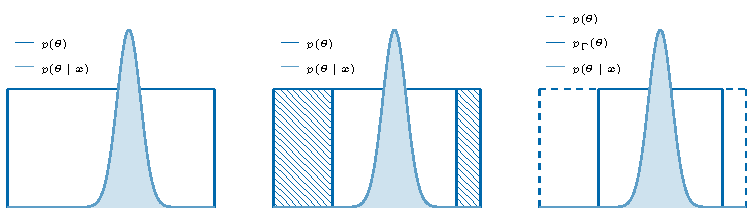
\includegraphics[width=\linewidth]{TikZ/truncation.pdf}
	\caption{Illustration of sequential inference for a 1-dimensional posterior. First, we learn an approximation to the posterior $p(\interest\mid\data)$ from the full initial prior $p(\interest)$. Then, we restrict the prior in the region where the parameter $\interest$ is likely to have generated $\data$. In the next inference round, the truncated prior $p_\Gamma(\interest)$ will be used to generate targeted simulations, sampling the parameter space more densely in the region of interest, so that the network can learn better in that region.}
	\label{fig:sbi-truncation}
\end{figure}

Importantly, since this sequential scheme does not modify the shape of the prior proposal distribution, but only restricts its support, the inference is still locally amortised in the constrained proposal distribution region, thus allowing for the possibility of tests that rely on performing inference across multiple observations (in the $\Gamma$ support). Moreover, it is also possible to use the same training data generated for a round to efficiently train arbitrary marginal posteriors for any set of model parameters. 

Training targeted ratio estimators is achieved by replacing the full prior with a \emph{truncated prior} $p^{(R)}_{\Gamma}(\interest)$, where the parameters are restricted to a region $\Gamma$ where they are likely to have generated $\data_0$. Since parameters from the complement of $\Gamma$ are unlikely to have generated $\data_0$, training a ratio estimator with data generated from the truncated prior as opposed to the full prior has little impact on the posterior learned by our ratio estimators. Indeed, only those regions where $p(\data_0 \mid\interest)$ is sufficiently negligible are removed, such that $p(\data_0\mid\interest) \to \mathbb{I}_\Gamma(\interest) \cdot p(\data_0\mid\interest)$ remains an accurate approximation for a given target observation $\data_0$. Indeed, too small values for the threshold $\epsilon$ are inefficient in focusing simulations, whereas too large values would cut into the relevant part of the posterior. For generous enough $\Gamma$, \ie\ an appropriate threshold $\epsilon$, the posterior remains essentially unchanged far into its tails,
\begin{equation}
\begin{split}
    p_\Gamma(\interest\mid\data) 
    &= \frac{p(\data\mid\interest)\,p_\Gamma(\interest)}{\int d\interest\, p(\data\mid\interest)\, p_\Gamma(\interest)}
    = \frac{p(\data\mid\interest)\,p(\interest)\cdot\mathbb{I}_\Gamma(\interest)\, V^{-1}}
    {\int d\interest\, p(\data\mid\interest)\,p(\interest)\cdot \mathbb{I}_\Gamma(\interest)\, V^{-1}} \\
    &\simeq \frac{p(\data\mid\interest)p(\interest)}{p(\interest)}
    = p(\interest\mid\data) \;. 
\end{split}
\end{equation}

%In practice, since the highest probability density region of the true posterior $\Gamma$ is unknown, we compute an estimate $\hat{\Gamma}$ over a sequence of inference rounds. At the beginning of each round, we sample from $p_{\hat{\Gamma}}(\interest)$ (or the full initial prior in the first round) and train a ratio estimator. We re-estimate $\hat{\Gamma}$ by keeping only the parts of the previous truncated prior for which $\hat{r}(\interest; \data)$ exceeds a certain threshold \cite{Miller:2021aa}. This determines the truncated prior for the next round. The final ratio estimator is obtained when $\hat{\Gamma}$ stops changing substantially between rounds, even when using more training data. 

This whole scheme relies on the assumption that posterior estimate $\hat p_{\Gamma}(\interest \mid \data_0)$ is a good approximation of $p(\interest \mid \data_0)$. An over-confident estimate would remove parameter ranges that are part of $\Gamma^{(R)}(\interest)$. In practice, this effect is not observed for a conservative choice of $\epsilon$. Moreover, one can test the convergence of the sequential scheme by checking whether high probability regions of the estimated posteriors intersect with the boundaries of the indicator function.


\subsection{Information maximizing neural network} \label{subsec:tmnre-nn}

From a practical perspective, a given inference involves training several classifiers (corresponding to the various marginal ratio estimators) in parallel. For complex and high-dimensional data, it is generally useful to compress it before it is input into the inference network through a so-called compression/summary/embedding network. Hence, the inference neural network usually employed to perform \gls*{tmnre} are generally split into two distinct components: an embedding network $C_\Phi(\data)$ and binary classification networks $d_\Phi(\data, \interest)$. 

The embedding network learns to compresses the potentially high-dimensional data into a low-dimensional feature vector, estimating the best possible summary statistics from the full input data, $\boldsymbol{s}= C_\Phi(\data)$. In principle, the compression network can be any sufficiently expressive network, no specialized network architectures are required. In practice, for faster convergence and better results specific inductive biases of different network architectures should be exploited, \eg~for image data, convolutional neural networks are often appropriate. Throughout this thesis, we will see various example of this (\eg~see Chapter~\ref{cha:lensing}). Furthermore, the compression network output can be shared as input to all of the classification networks, or subdivided between the classifiers, in order for each compressed summary to be optimized for the specific marginal estimator. 

While the purpose of the embedding network is to efficiently summarize data, the purpose of classifiers $d_\Phi(\boldsymbol{s}, \interest)$ is to learn the correlation between the data summary $\boldsymbol{s}$ and the parameters of interest $\interest$ in order to perform the actual ratio estimation. Their inputs are the learned summaries of the observational data concatenated with the parameters of interest for the targeted marginal. Usually, the classifiers are parameterized with fully connected layers and unless otherwise specified in this thesis we will be using the ResNet \cite{he2016deep} architecture as implemented in \swyft \cite{Miller2022}.

The compression network and ratio inference are \emph{optimized simultaneously}, in contrast to other algorithms in the literature, minimizing the \gls*{bce} loss function (Equation~\eqref{eq:sbi-bce-m}). The structure of a general network architecture can be expressed as:
\begin{equation}\label{eq:nn-c}
    d_\Phi(\boldsymbol{s}= C_\Phi(\data), \interest) \simeq  d_\Phi(\data, \interest)  = \sigma[ \log \hat{r}(\interest; \data)] \;.
\end{equation}
%and is illustrated in Figure~\ref{fig:sbi-nn}.

%\begin{figure}
%    \centering
%	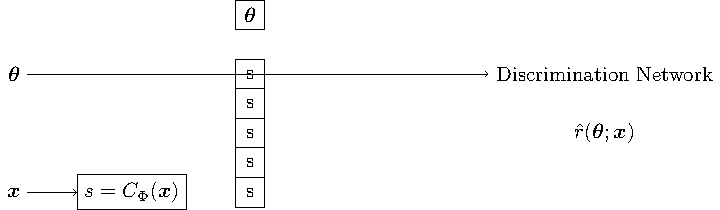
\includegraphics[width=\linewidth]{TikZ/sbi_nn.pdf}
%    \caption{\todo{Finish} Illustration of the network architecture, including the embedding network $C_\Phi(\data)$ and the discrimination network $d_\Phi(\boldsymbol{s}, \interest)$. Input data $\data$ and parameters $\interest$ are internally mapped to the marginal parameter combinations of interest, for which individual ratio estimators with a shared compression network are trained. The outputs are estimated ratios for the marginal posteriors of interest... \todo{Finish}}
%    \label{fig:sbi-nn}
%\end{figure}


It is interesting to understand why the approximately equal sign in Equation~\eqref{eq:nn-c} holds and which features $\boldsymbol{s}$ are learned by the embedding network during training, \eg~in comparison to the hand-crafted ones employed in \gls*{abc} (Section~\ref{sec:sbi}). Following Ref.~\cite{Cole:2021gwr}, the \gls*{bce} loss in Equation~\eqref{eq:sbi-bce-m} can be written in terms of the Jensen-Shannon divergence (JSD) as
\begin{equation}
   \mathcal{L}[d_{\bm{\Phi}}(\data, \interest)] = 2 \log2 - 2\mathbb{E}_{p(\data)}\left[D_{JS}(p(\interest\mid\data)\| p(\interest)\right] \;,
\end{equation}
which follows\footnote{
   In fact,
   \begin{multline}
   -2\mathbb{E}_{p(\data)}\left[D_{JS}\left(p\left(\interest\mid\data\right) \parallel  p(\interest)\right)\right] \\
   =-\mathbb{E}_{p(\data)}\left[
      D_{KL}\left(p\left(\interest\mid\data\right) \parallel \frac12\left(p\left(\interest\mid\data\right) + p(\interest)\right)\right)
      +D_{KL}\left(p\left(\interest\right) \parallel \frac12\left(p\left(\interest\mid\data\right) + p(\interest)\right)\right)\right]\\
   = -\int d\data\, d\interest\,
   \underbrace{p(\data)p(\interest\mid\data)}_{\to p(\data, \interest)} \ln \frac{p\left(\interest\mid\data\right) }{ \frac12\left(p\left(\interest\mid\data\right) + p(\interest)\right)}
   +p(\data)p(\interest) \ln \frac{p\left(\interest\right) }{ \frac12\left(p\left(\interest\mid\data\right) + p(\interest)\right)}\\
   = -\int \dd{\data} \dd{\interest} \left\{ p(\data, \interest) \log d_{\bm{\Phi}}(\data, \interest) \notag + p(\data) p(\interest) \log\left[ 1 - d_{\bm{\Phi}}(\data, \interest) \right] \right\} \\
   = \mathcal{L}[d_{\bm{\Phi}}(\data, \interest)] - 2\ln 2 \;,
\end{multline}
where the third equation follows from Equation~\eqref{eq:sbi-classifier}.
}
directly from the definition of the JSD
\begin{equation}
    D_{JS}(p\| q) = \frac{1}{2}D_{KL}(p \parallel m)+\frac{1}{2}D_{KL}(q \parallel m)\;,
\end{equation}
where $m=(p+q)/2$ and $D_{KL}$ denotes the Kullback-Leibler divergence, $D_{KL}(p(x) \mid q(x) = \int \dd x p(x) \log\left(\frac{p(x)}{q(x)}\right)$.

We can now apply the same logic to our network with a compression step, an information bottleneck, in Equation~\eqref{eq:nn-c}. The posterior is then conditioned on the summary statistics $\boldsymbol{s}$, and the loss function can be written as
\begin{equation} \label{eq:loss-jsd}
   \mathcal{L}[d_{\bm{\Phi}}(\boldsymbol{s} = C_\phi(\data), \interest)] = 2 \log2 - 2\mathbb{E}_{p(\data)}\left[D_{JS}(p(\interest\mid\boldsymbol{s} = C_\phi(\data))\| p(\interest)\right] \;.
\end{equation}
%thus, data summaries $\boldsymbol{s}$ are learned such that they maximize the JSD between posteriors and priors.  

Looking at Equation~\eqref{eq:loss-jsd}, assuming a fully converged classifier and the loss as a function of the summary $\boldsymbol{s}$, it becomes now evident that a data summary $\boldsymbol{s}$ that minimizes the \gls*{bce} loss has to \emph{maximize} the expected JSD between the data-summary-based posterior and the prior for the parameters of interest $\interest$. Therefore, data summaries $\boldsymbol{s}$ that sufficiently describe data $\data$ for a parameter $\interest$ lead to posteriors $p(\interest\mid\data)$. On the other hand, inefficient data summaries will lead to wider posteriors which are more similar to the prior, reducing the JSD, and increasing the value of the loss function.  Hence, it makes sense to expect that the data summaries that are learned are the most informative to discriminate between samples from the posterior and the prior, or, equivalently, to discriminate whether the likelihood-to-evidence ratio is larger or smaller than one,
\begin{equation}
    \frac{p(\boldsymbol{s} \mid \interest)}{p(\boldsymbol{s})}  = 
    \frac{p(\interest\mid \boldsymbol{s})}{p(\interest)} 
    \lessgtr 1\;.
\end{equation}


%What does a large JS-divergence signify? To see this, we consider the average Bayesian probability of error of wrongly classifying a parameter-data pair as drawn from the prior or the posterior, which is given by
%%
%\begin{equation}
%    \hat P_e = \mathbb{E}_{\data \sim p(\data)} \left[\frac12 \min(p(\interest\mid\data), p(\interest))\right]
%\end{equation}
%%
%In Ref.~\cite{XYZ} it was shown that the minimum of the NRE loss provides an upper bound on the error rate,
%%
%\begin{equation}
%    \hat P_e
%    \leq
%    2\log 2 -  
%    2 \mathbb{E}_{\data\sim p(\data)}\left[D_{JS} ( p(\interest\mid\data) \;\|\; p(\interest))\right]
%    \leq \ell_{NRE}[F_\phi]\;.
%\end{equation}
%
%When using NRE as described above, the summary is optimized such that it minimizes (an upper bound on) the error rate when classifying points as drawn from the prior vs. drawn from the posterior, or (equivalently) whether the likelihood-to-evidence ratio is larger or smaller than one,
%%
%\begin{equation}
%    \frac{p(\boldsymbol{s} \mid \interest)}{p(\boldsymbol{s})}  = 
%    \frac{p(\interest\mid \boldsymbol{s})}{p(\interest)} 
%    \lessgtr 1\;.
%\end{equation}

%\subsection{Hierarchical inference} \label{subsec:tmnre-hierarchical}
%\todo{Add brief paragraph about hierarchical inference in SBI to setup the problem for populations of subhalos in lensing and point sources in maps?} 
%
%When analyzing real-world data it is common to work with event ensembles, which comprise sets of observations that collectively constrain the parameters of an underlying model of interest. Such models often have a hierarchical structure, where “local” parameters impact individual events and “global” parameters influence the entire dataset. 
%Datasets composed of multiple samples are ubiquitous in scientific and more broadly real-world data analysis tasks. These datasets are typically governed by underlying models that exhibit a rich hierarchical structure, with local parameters shaping individual events while global parameters exert influence across the entire dataset. This layered structure, if appropriately utilized, can greatly augment the efficiency and effectiveness of the inference process.
%We substantiate theoretically as well as empirically the fact that hierarchy-aware inference in many implicit models with a hierarchical structure requires a dataset-wide approach, contrasted with the more common paradigm of combining implicit likelihood or posterior estimators associated with individual observations.
%
%The joint probability distribution of a set of events with cardinality N, with global parameters of interest \interest, global nuisance parameters \interestν as well as local parameters zi can be written as:
%N
%p({x} | {z},\interest,\interestν) = Yp(xi | zi,\interest,\interestν), (1)
%i=1
%
%come from different stellar populations have different intrinsic prop
%Hierarchical Bayesian modelling, however, comes at the cost of having to infer individual parameters for each observed SN Ia, and so the computational burden scales with the data set size
% population variability 
%perform simulation-based inference over event ensembles and can deal with datasets of varying cardinality\cite{Heinrich:2023bmt}

\clearpage

\begin{figure}
	\centering
	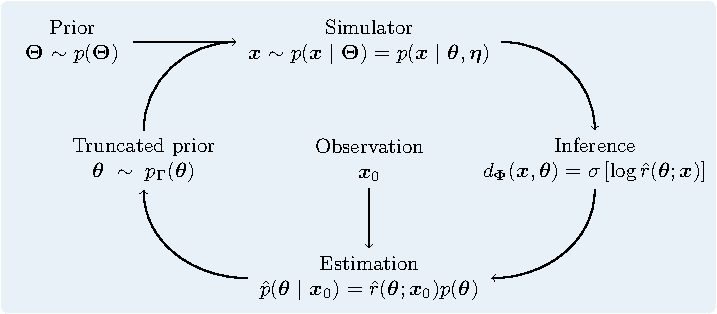
\includegraphics[width=\linewidth]{TikZ/tmnre.pdf}
	\caption{\textbf{Truncated marginal neural ratio estimation.} Parameters, both of interest $\interest$ and nuisance $\nuisance$, are sampled from the initial prior $p(\param)$, and mapped into data $\data$ through a programmed simulator that effectively acts as in implicit likelihood. Inference is performed by training binary classifiers $d_\Phi(\data, \interest)$ with marginal \gls*{nre} to learn the estimates of the ratios of interest $\hat{r}(\interest;\data)$ (Sections~\ref{subsec:tmnre-nre} and \ref{subsec:tmnre-m}). The ratios are used to weight prior samples, enabling posterior sampling for any observation $\data$. Focusing on a target observation $\data_0$, we can perform sequential inference (Section~\ref{subsec:tmnre-t}) via prior truncation, by constraining the initial parameter space for the inferred parameters to regions $\Gamma^{(R)}(\interest)$ that are most relevant for a specific target observation $\data_0$. The procedure is repeated until convergence.
}
\label{fig:sbi-tmnre}
\end{figure}

In this section we have introduced the technical details of the \gls*{tmnre} algorithm, and its key building blocks: \gls*{nre} (Section~\ref{subsec:tmnre-nre}), marginalization  (Section~\ref{subsec:tmnre-m}), and prior truncation  (Section~\ref{subsec:tmnre-t}). We have also seen the general network architecture that is usually employed within this algorithm (Section~\ref{subsec:tmnre-nn}). A complete sketch of the workflow of a \gls*{tmnre} algorithm is illustrated in Figure~\ref{fig:sbi-tmnre}. We will see in Section~\ref{sec:test} how to test its results.



\section{Testing SBI: getting it right} \label{sec:test}

\gls*{tmnre} is a \emph{locally amortized} technique, meaning that the ratio estimator are trained to learn a function, that can then be evaluated to perform inference very quickly on \emph{any} number of data, thanks to the great evaluation speed of neural networks. This opens up the possibility to perform consistency checks of the statistical properties of the trained networks, within the constrained region over which they have been trained, in each stage of truncation. These type of tests are generally infeasible for likelihood-based methods, where the algorithms perform inference on a single fixed observation and must rerun from scratch for another observation. In this likelihood-based settings, it is hence computationally very costly to test coverage on simulated data, and usually the statistical properties of the inference results are instead inferred based on convergence criteria of the sampling chains \cite[\eg][]{vivekan2019convergence}. This difference is illustrated in Figure~\ref{fig:sbi-test}.

Using local amortization, one can cheaply validate the Bayesian coverage properties of the approximate posteriors \cite{Hermans:2021rqv, Cole:2021gwr, Karchev:2022xyn}, and construct confidence regions with exact frequentist coverage \cite{Karchev:2022xyn, dalmasso2020confidence, dalmasso2021likelihood}. Here we focus on the former types of tests, and use the \emph{expected coverage test} that probes the empirical (\ie~determined from analyses of simulated data $\data$) Bayesian coverage properties of the estimated posteriors $\hat{p}(\interest \mid \data)$.

An \emph{expected coverage test} measures whether Bayesian credible regions of different widths, $\Omega_{p(\interest \mid \data)}(1-\alpha)$, have achieved their $1-\alpha$ nominal coverage \cite{Hermans:2021rqv, Cole:2021gwr}. In simple words, it checks whether the true parameters $\interest$ fall within the credible region, of the estimated posterior $\hat{p}(\interest\mid\data)$ for $\alpha\%$ of the randomly drawn observations $\data \sim p(\data\mid\interest)$:
%
\begin{align}
	1-\hat{\alpha} &\equiv \mathop{\mathbb{E}}\limits_{p(\data, \interest)} \left[ \mathbb{I} \left[ \interest \in \Omega_{\hat{p}(\interest \mid \data)}(1-\alpha) \right] \right] \\
		& \mathop{\rightarrow}\limits_{\hat{p} \rightarrow p}  \mathop{\mathbb{E}}\limits_{p(\interest)} \underbrace{\mathop{\mathbb{E}}\limits_{p(\interest\mid\data)} \left[ \mathbb{I} \left[ \interest \in \Omega_{p(\interest \mid \data)}(1-\alpha) \right] \right]}_{ = 1-\alpha}.
\end{align}
%
In the limit where the estimator $\hat{p}(\interest\mid\data)$ approaches the correct one ${p}(\interest\mid\data)$, one trivially expect that $1-\alpha=1-\hat{\alpha}$. 

\begin{figure}
	\centering
	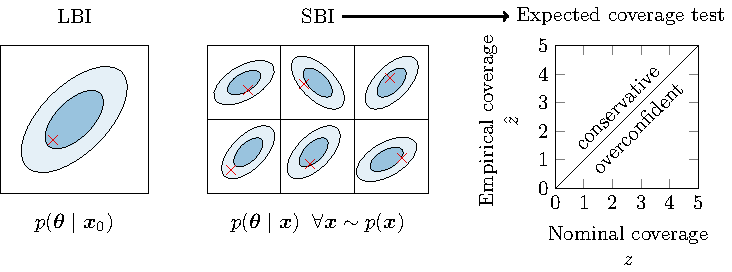
\includegraphics[width=\linewidth]{TikZ/sbi_test.pdf}
	\caption{Testability: Contrary to \gls*{lbi} algorithms, many \gls*{sbi} methods, including \gls*{tmnre}, do not estimate just a single posterior, but all of them simultaneously. This property is called ``amortization" in the machine learning field \cite{amos2023tutorial}. Amortization enables the user to efficiently test the reliability of the inference results, for example with expected Bayesian coverage tests ({rightmost panel}). The left part of the figure is inspired and adapted from Figure 4 in Ref.~\cite{Cole:2021gwr}.
}
\label{fig:sbi-test}
\end{figure}


In case of a conservative estimator, the nominal credibility $1-\alpha$ is lower than the empirical one $1-\hat\alpha$, and vice versa for an overconfident estimator. In general, in case of a conservative coverage plot one should check if the estimator has fully converge. On the other hand, in case of an overconfident coverage plot, one should check for overfitting. In combination with visually checking the posteriors, this test supports the accuracy of the posterior estimator and is also particularly useful when one does not have access to the ground truth against which to compare the results. 

Agreement between the nominal and empirically-measured expected coverage is a necessary (but not sufficient) condition for the density/ratio estimator to be a correct estimate of the posterior. Indeed, the expected coverage test checks for the consistency of the posterior, not for its precision. For example, a not focused posterior that resembles the prior leads to a diagonal plot with optimal coverage. Moreover, it tests for the coverage \emph{averaged} over parameter values $\interest \sim p(\interest)$. As a result, some parameter regions might be over- and other parameter regions under-covered.

Since we are mostly interested in small values of $\alpha$, corresponding to posterior regions with high mass, it is convenient to reparameterize $\alpha$ in terms of a new variable $z$, defined as $1-\frac12 \alpha$ quantile of the standard normal distribution \cite{Cole:2021gwr}. As a results,  $z = 1, 2, 3$ have $1-\alpha = 0.6827, 0.9545, 0.9997$, and correspond to the common $1\sigma$, $2\sigma$, $3\sigma$ regions. We show a mock example of such test in the right panel of in Figure~\ref{fig:sbi-test} to illustrate its general behavior.


In Chapter~\ref{cha:lensing}, we will use empirical coverage plots in order to double-check and confirm the convergence of our posterior estimators for strong lensing image analysis. Closely related versions of this test and plots have appeared in the literature, \eg~in Refs.~\cite{Dax:2021tsq,Karchev:2022xyn, Bhardwaj:2023xph}. Developing more tests in order to trust results generated by \gls*{sbi} algorithms is very active and ongoing work \cite{linhart2024c2st, lemos2023sampling}. For example, it is worth mentioning an alternative method of defining Bayesian credible regions using distances to random points, which can, in certain circumstances, detect a systematic bias \cite{lemos2023sampling}.


\section{Neural SBI methods comparison} \label{sec:comparison}

Each of the three core neural \gls*{sbi} algorithms described in Section~\ref{subsec:nsbi} has its distinct benefits and drawbacks. The most suitable choice between \gls*{npe}, \gls*{nle}, and \gls*{nre} is largely determined by the properties of the underlying problem, the dimensions of the data and of the parameter space, and the specific application. For a quantitative comparison of the three algorithms on machine learning benchmarks, we refer the reader to Ref.~\cite{Lueckmann:2021aa}. In this section, following discussions from Refs.~\cite{Cranmer:2019eaq, Cole:2021gwr, Ho:2024whi}, we focus on describing qualitative similarities and differences between them.

In general, \gls*{npe} and \gls*{nle} solve a density-estimation problem via an \emph{unsupervised} learning task, as there are no explicit labels. Instead, \gls*{nre} solves a classification problem via a \emph{supervised} learning task, which is often simpler. Moreover, ratios can be estimated with simple classification networks, which are often easier to train than density estimation models (as normalizing flows). Hence, for higher-level inference, learning an estimator for the likelihood-ratio function may often be more efficient.

Furthermore, density estimation becomes increasingly hard when the dimension of the data is large, or the data distribution is highly complex \cite{papamakarios2021normalizing}. This problem is alleviated by compressing the data to some simple low-dimensional summary statistics before performing inference with density estimators. For example, a compression network, such as an Information Maximizing Neural Network \cite{charnock2018automatic}, is often used. The \emph{compression} network is typically trained upfront before inference, with additional simulation cost. On the other hand, as seen in Section~\ref{subsec:tmnre-nn}, in \gls*{nre} the compression network and the ratio estimator are trained simultaneously.    	 

One of the key advantages of \gls*{npe} and \gls*{nle} over \gls*{nre} is the additional \emph{sampling functionality} from the surrogate model, which is not possible for \gls*{nre} parameterized via \eg\ a \gls*{mlp}. For \gls*{nre} and \gls*{nle}, one needs a way to sample from the neural posterior after training. Still, likelihood(-to-evidence ratio) evaluation is generally very fast thanks to the massive evaluation speed and parallelization afforded by neural networks. Broadly, \gls*{npe} models are better suited for scenarios requiring repeated inference across multiple observations, as it can be prohibitively expensive to run sampling chains for \gls*{nre} and \gls*{nle} for many test points. On the other hand, for hierarchical likelihood sampling, \gls*{nre} and \gls*{nle} will be a more effective choice.

Despite these initial differences, the three algorithms share many similarities. First of all, when not using active learning, all three approaches are \emph{amortized}: after an upfront simulation and training phase, they can all be efficiently evaluated for arbitrary data and parameter points (in the prior support). Second, all three approaches can use \emph{active learning}, iteratively updating the proposal distribution to guide the simulator parameters toward the relevant parameter region (Section~\ref{subsec:tmnre-t}).

It is also important to note that, while \gls*{npe} directly targets the posterior, it induces a prior dependence in the inference. On the other hand, \gls*{nre} and \gls*{nle} are prior independent, allowing extra flexibility to change the prior during inference, and the possibility to do frequentist inference or model comparisons. 
	
While all approaches can directly target marginal posteriors \cite{Miller:2020hua, Miller:2021aa, Alsing:2019dvb, Jeffrey:2020itg}, some extra care is required when combining marginalization and active learning if there is a prior dependence in the inference. Indeed, marginal estimation will be in general affected by the proposal distribution, since one implicitly integrates over it. This generally cannot be undone after training (for a workaround where marginalization can be integrated into the compression step by constructing appropriate summary statistics see, \eg, Ref.~\cite{Alsing:2019dvb}). 

Combining the insights from all algorithms, which are currently categorized as distinct, is expected to lead to facilitate further advancements.


\section{SBI applications in this thesis} \label{sec:applications}

In this first chapter, we have learned about the benefits of simulation-based analysis for data inference, and particularly about the \gls*{tmnre} algorithm. In the next chapters, we will see its applications to various astrophysical problems: the analysis of strong gravitational lenses as a dark matter probe (Chapter~\ref{cha:lensing}), how to scale it to higher dimensional problems with more correlated parameter spaces (Chapter~\ref{cha:anre}), the reconstruction of cosmological initial conditions Chapter~\ref{cha:cosmo}), and the analysis of a population of point-sources in sky-maps (Chapter~\ref{cha:detection}). The common thread between all these applications is being formally representable by \emph{large and complex forward models}, with many moving parts, on a subpart of which we would like to perform precise scientific inference while correctly propagating uncertainties from the others. This is possible in a \gls*{sbi} framework.

In particular, we will see many of the several types of marginal posteriors that can be directly inferred in simulation-based settings, and which answer specific inference questions relevant for the application at hand. Some of the marginal quantities we will encounter in the different chapters of this thesis are:
\begin{itemize}[leftmargin=1cm]
	\item posterior of a single parameter (Chapters~\ref{cha:lensing}, \ref{cha:anre}, and \ref{cha:detection});
	\item 2-dimensional posteriors of parameter pairs (Chapters~\ref{cha:lensing}, \ref{cha:anre}, and \ref{cha:detection});
	\item n-dimensional posteriors of parameters (Chapter~\ref{cha:anre});
%	\item posterior for discrete (categorical) variables that label model choices
	\item posterior probability of a pixel value for field reconstruction (Chapter~\ref{cha:cosmo});
    \item posterior probability of an object being present in a specific image region (Chapter~\ref{cha:detection});
	\item posterior for the number of objects in an image  (Chapter~\ref{cha:lensing} and \ref{cha:detection}).
\end{itemize}


Moreover, prior truncation will be achieved by means of different strategies of increasing complexity throughout all of these applications, depending on the their specificities. The main strategies we will see are:
\begin{itemize}[leftmargin=1cm]
	\item 1-dimensional box truncation (Chapters~\ref{cha:lensing}, \ref{cha:anre}, and \ref{cha:detection});
	\item n-dimensional hard-likelihood truncation with nested sampling  (Chapter~\ref{cha:anre});
	\item truncation with tempered likelihood  (Chapter~\ref{cha:cosmo});
	\item object detection as prior truncation  (Chapter~\ref{cha:detection}).
\end{itemize}

A detailed contextualization and explanation of the technicalities of each strategy will be given in the respective chapters. 







